\chapter{Design}

This chapter contains a high level description of the design choices made in the process of creating Viskell.
The specific implementation details are discussed in chapter \ref{chap:implementation} on page \pageref{chap:implementation}.

\section{User interface}

The user interface basically consists of two parts, namely the menus for the different options a user can select and the part where the user can manipulate functions and create their own (the \gls{canvas}). \index{canvas}

\subsection{Graphical design}

\subsubsection{Blocks and lines}

We chose to represent Haskell functions by function blocks since this is a logical element for users, a combination of blocks forms a program.
Each block consists of a function name and its associated arguments. With each argument comes an anchor node to which other block can be connected through lines.

In Haskell, values are passed to functions without being saved as variables.
The lines between blocks represent this flow.
Thus, a program can be built like an electronic circuit.

We chose to make a distinction between three kinds of blocks.
The first kind in an input block, which represents a constant value. \index{value block} \index{input block}
This input block can be connected to other blocks to use the value as an input.
Besides the most basic input block, the value block which takes a string as input and automatically detects the type, there is also a slider available. \index{slider block}

\begin{figure}[p]
	\centering
	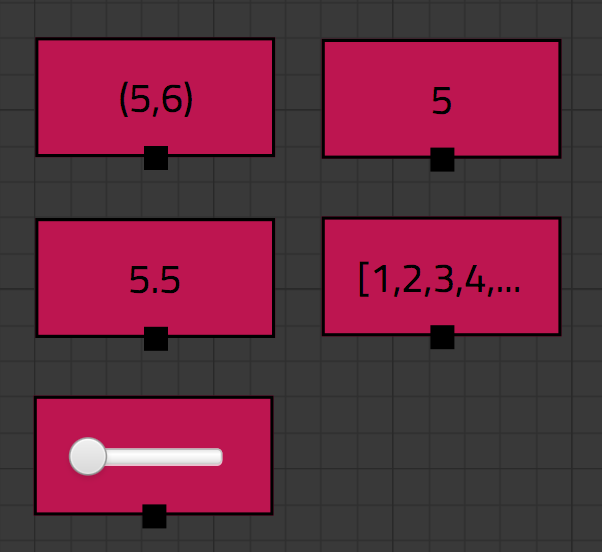
\includegraphics[scale=0.5]{Images/blocks-inputs}
	\label{fig:blocks-inputs}
	\caption{Different input blocks}
\end{figure}

The second kind of block is a function block. This block has a number of inputs and a single output, and defines the number of inputs that are going to be used. \index{function block}
The number of inputs can be changed by moving a knot over the function arguments.
This allows for passing (partially applied) functions as input for other functions. \index{partial application}
A useful example for this is the \code{map} function.

\begin{figure}[p]
	\centering
	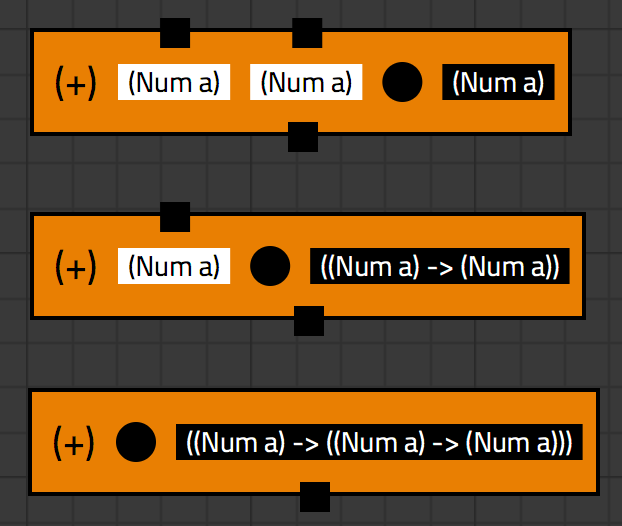
\includegraphics[scale=0.5]{Images/blocks-bowties}
	\label{fig:blocks-bowties}
	\caption{Partial application of functions}
\end{figure}

The third kind of block displays an output.  \index{output block}
There are multiple versions, ranging from a simple block that displays the string representation to a graph block which can show a function. \index{graph block}

\begin{figure}[p]
	\centering
	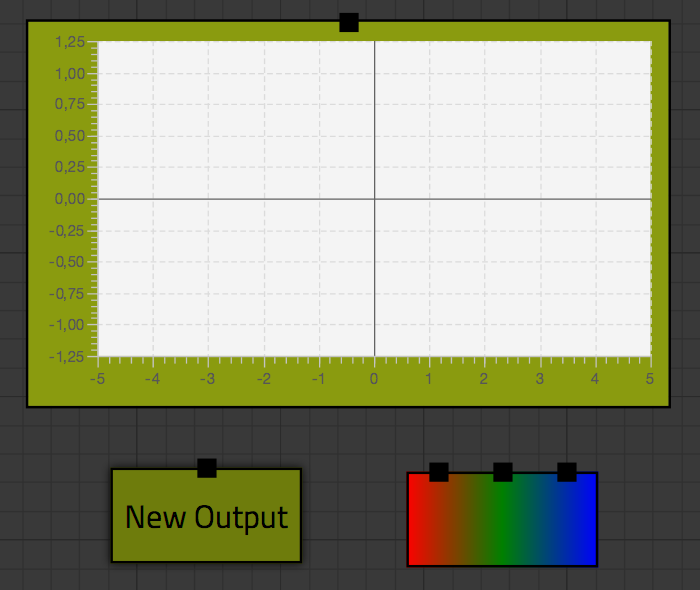
\includegraphics[scale=0.5]{Images/blocks-outputs}
	\label{fig:blocks-outputs}
	\caption{Different output blocks}
\end{figure}

Each kind of block has a different color to make them easily recognizable.
% Not entirely correct

\begin{figure}[p]
	\centering
	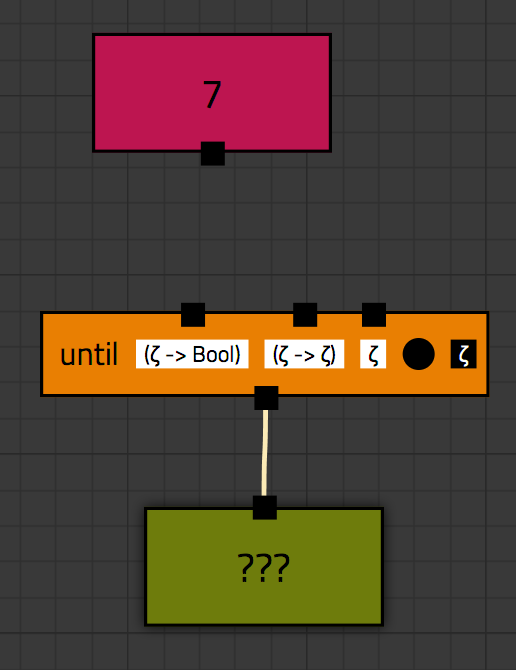
\includegraphics[scale=0.5]{Images/blocks-example}
	\label{fig:blocks-example}
	\caption{Different kinds of blocks}
\end{figure}

\subsubsection{Errors}

An important part of Viskell is representing programming errors.
Instead of requiring users to compile a complete program, type errors are displayed as soon as a user connects two blocks.
An error is represented as a colored line and colored type in the target block.
An icon is displayed as well to help color blind users.

\subsubsection{Menus}

During the design process many ideas for the menus came up.
One of the first ideas was to have a circular menu. \label{circular_menu} \index{circle menu}
The advantages of the circle menu would be that the orientation of the device would not have any influence on the usability of the menu.
This makes using the program on a large multi-touch table easier.
However, the implementation of the menu would take too much time and the idea was therefore dismissed.

\begin{figure}[p]
	\centering
	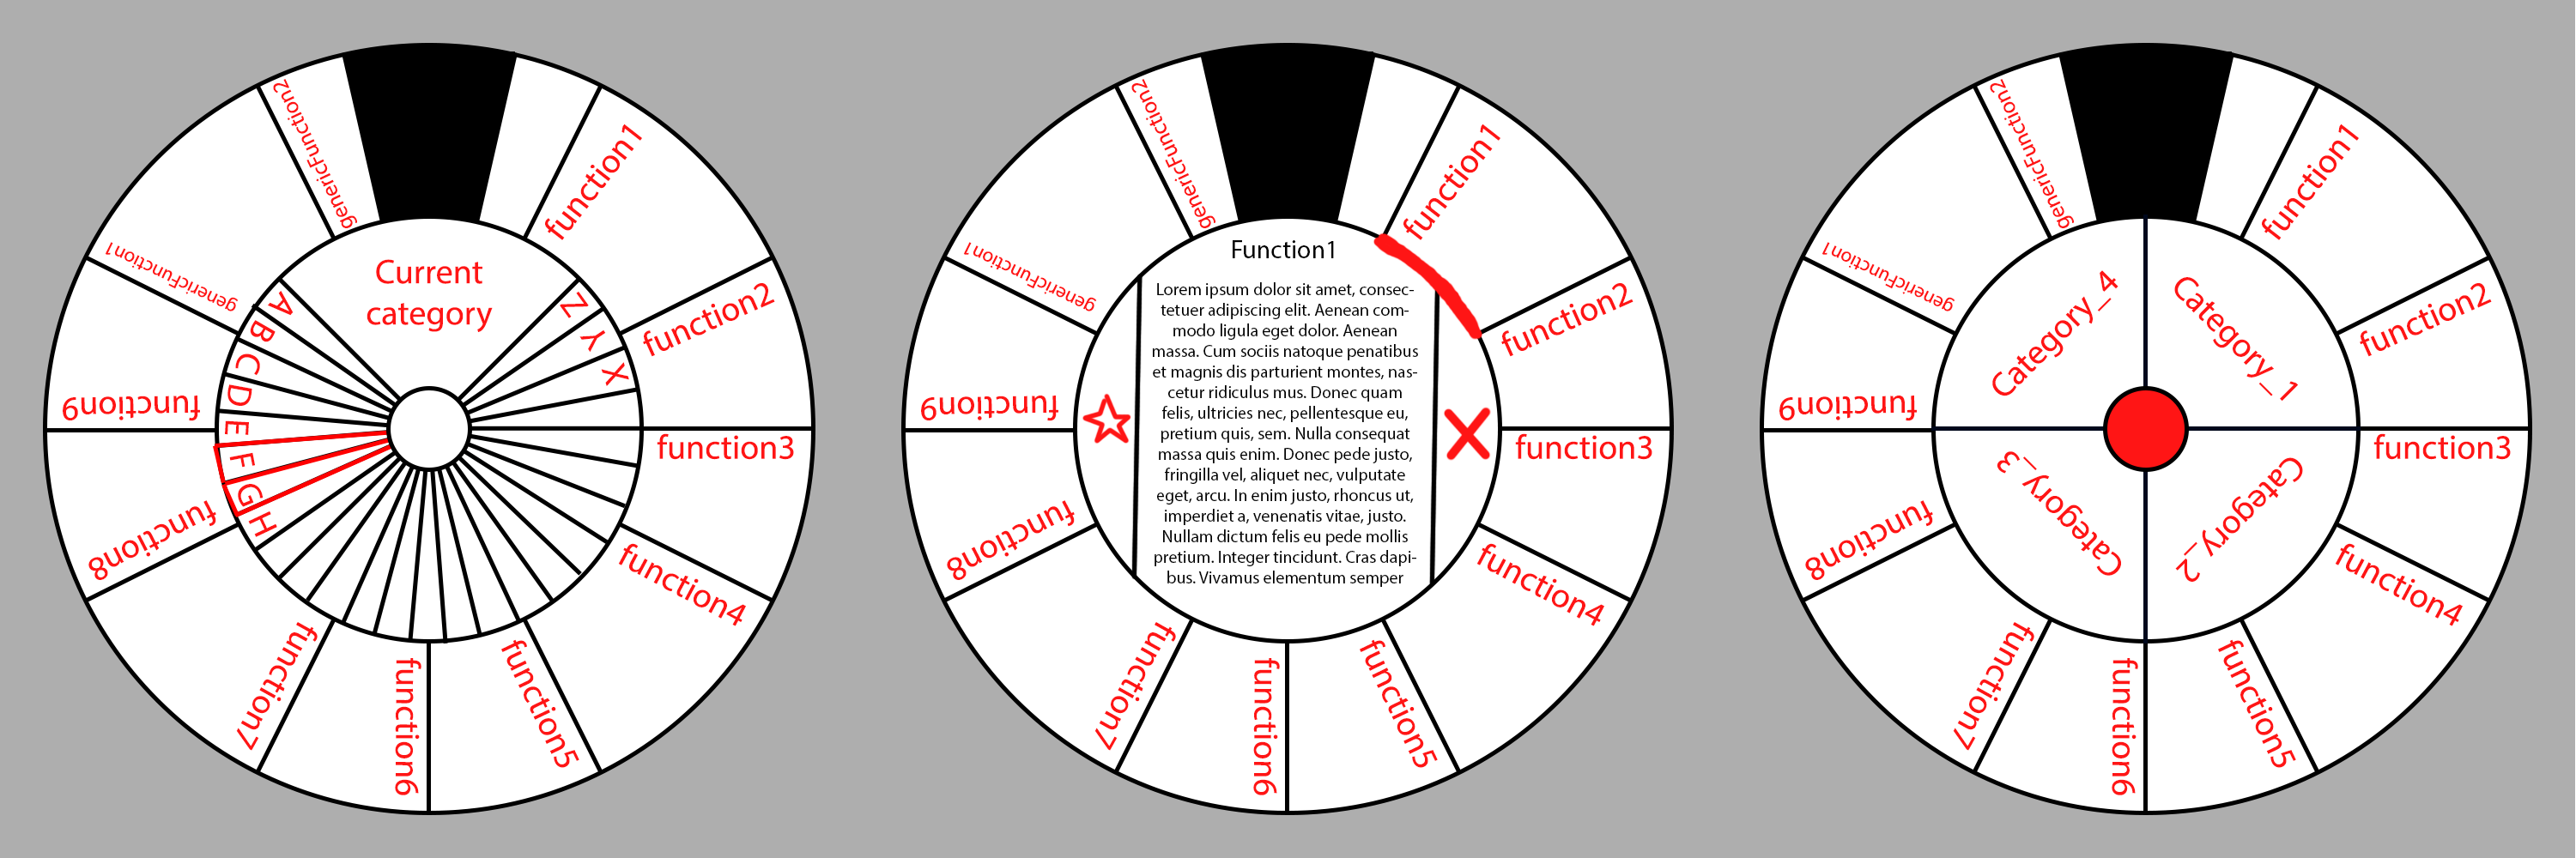
\includegraphics[width=\textwidth]{Images/circlary}
	\label{fig:circlary}
	\caption{Concept of circular menu}
\end{figure}
\begin{figure}[p]
	\centering
	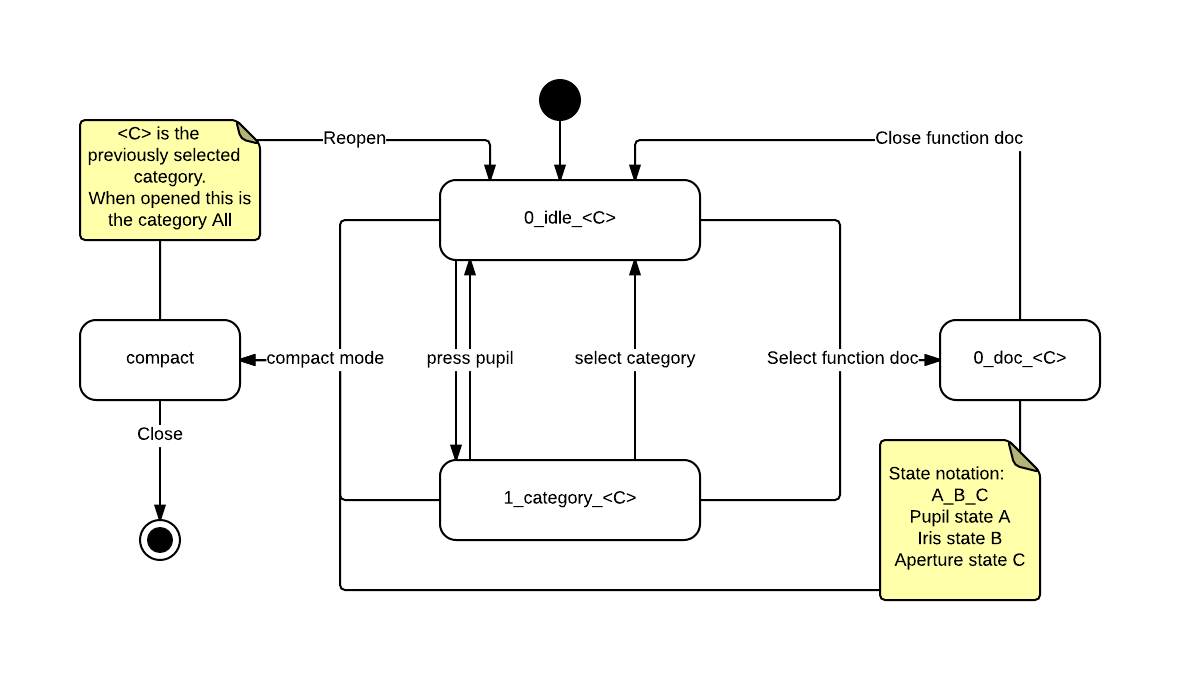
\includegraphics[scale=0.5]{Images/diagram-circlary}
	\label{fig:diagram-circlary}
	\caption{Circular menu diagram}
\end{figure}

The final design has two separate menus, one for adding new blocks and one for options on existing blocks.

The primary menu (or `function menu') uses `drawers' for the categories of the functions. \index{primary menu} \index{function menu}
This way it is easy to find functions even without an extensive knowledge of Haskell.
In- and output blocks and the function definition block can be created using buttons at the bottom of the menu.
This location is chosen to make them quickly available.
The primary menu can be opened multiple times at once and moved around the screen so multiple users can work on a single program.
% And not limited by the size of the screen.

\begin{figure}[p]
	\centering
	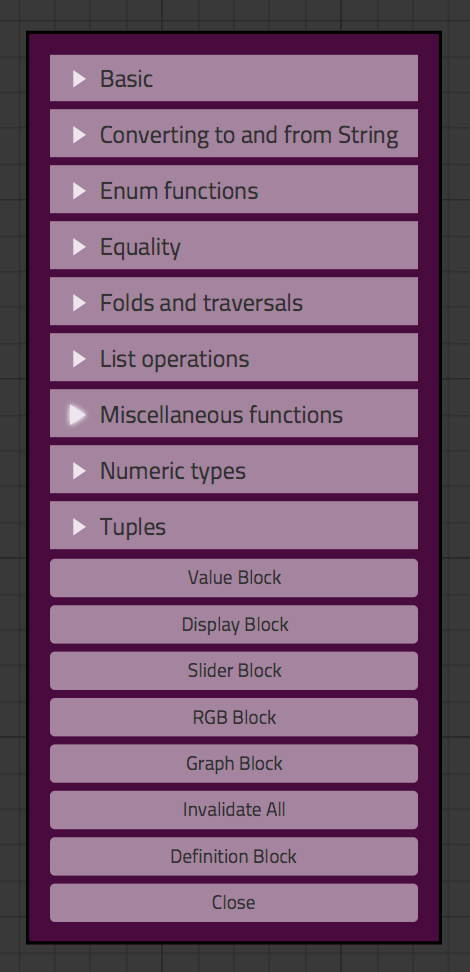
\includegraphics[scale=0.5]{Images/menu}
	\label{fig:ui-menu}
	\caption{Primary menu}
\end{figure}

The context menu is compact so is does not take up too much space. \index{context menu}
It contains clear icons which represent different actions for that single block, like delete.
The icons are large enough to touch, even for people with large fingers.

\begin{figure}[p]
	\centering
	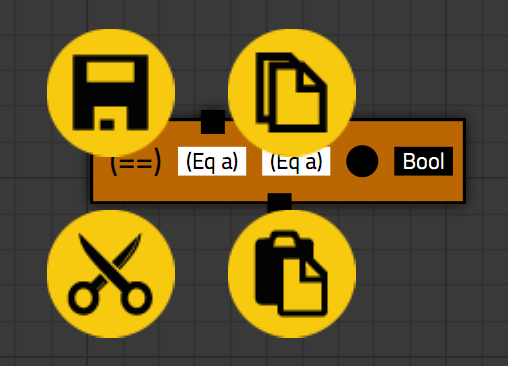
\includegraphics[scale=0.5]{Images/blocks-menu}
	\label{fig:blocks-menu}
	\caption{Context menu}
\end{figure}

\subsubsection{Color scheme}

The background color is a dark gray.
This is chosen because it is less tiring for the eyes than white and allows for a high contrast.
The background also incorporates a grid pattern so users can align elements on the screen if they like to.

All other components feature a cheerful color scheme.
This color scheme provides good contrast with the background and good recognizability for the different kinds of blocks.

\subsection{Behaviour and interaction design}

Interaction with the user interface is possible through touch gestures on the touch screen and on mouse actions on the computer.
We wanted the application to be very easy to use.
Since JavaFX only supports three different touch events, we decided to only use the matching gestures drag, tap and tap-hold (or right click on a computer).
With these three gestures everything is accessible in the program.
More complicated gestures were considered, but implementation proved to be difficult, especially with multiple users in mind.

We also wanted the user to have to perform as little unnecessary actions to complete an action.
An example is that a user does not have to disconnect a line first but can connect a new line to a connected anchor, which will automatically disconnect the old line.
Also, users are able to restore opening the context-menu by just clicking somewhere else.

Providing the possibility to easily spot the result of an action and undo wrong actions helps to keep the learning curve of the program flat and the behavior of the program predictable.

In the figure \ref{fig:activitydiagram} on page \pageref{fig:activitydiagram} it is shown that the number of actions a user can perform is not very large. This results in a short learning curve, as mentioned before. Although the number of actions is not very large, the number of possibilities in the program at a given point is quite extensive. This is visualised by the many lines in the activity diagram.

We also kept in mind that the program might have to be usable for multiple users at the same time in the future; we made it possible to open multiple menus at the same time. Different users can also perform the same or different gestures at the same time.

\begin{figure}[p]
	\centering
	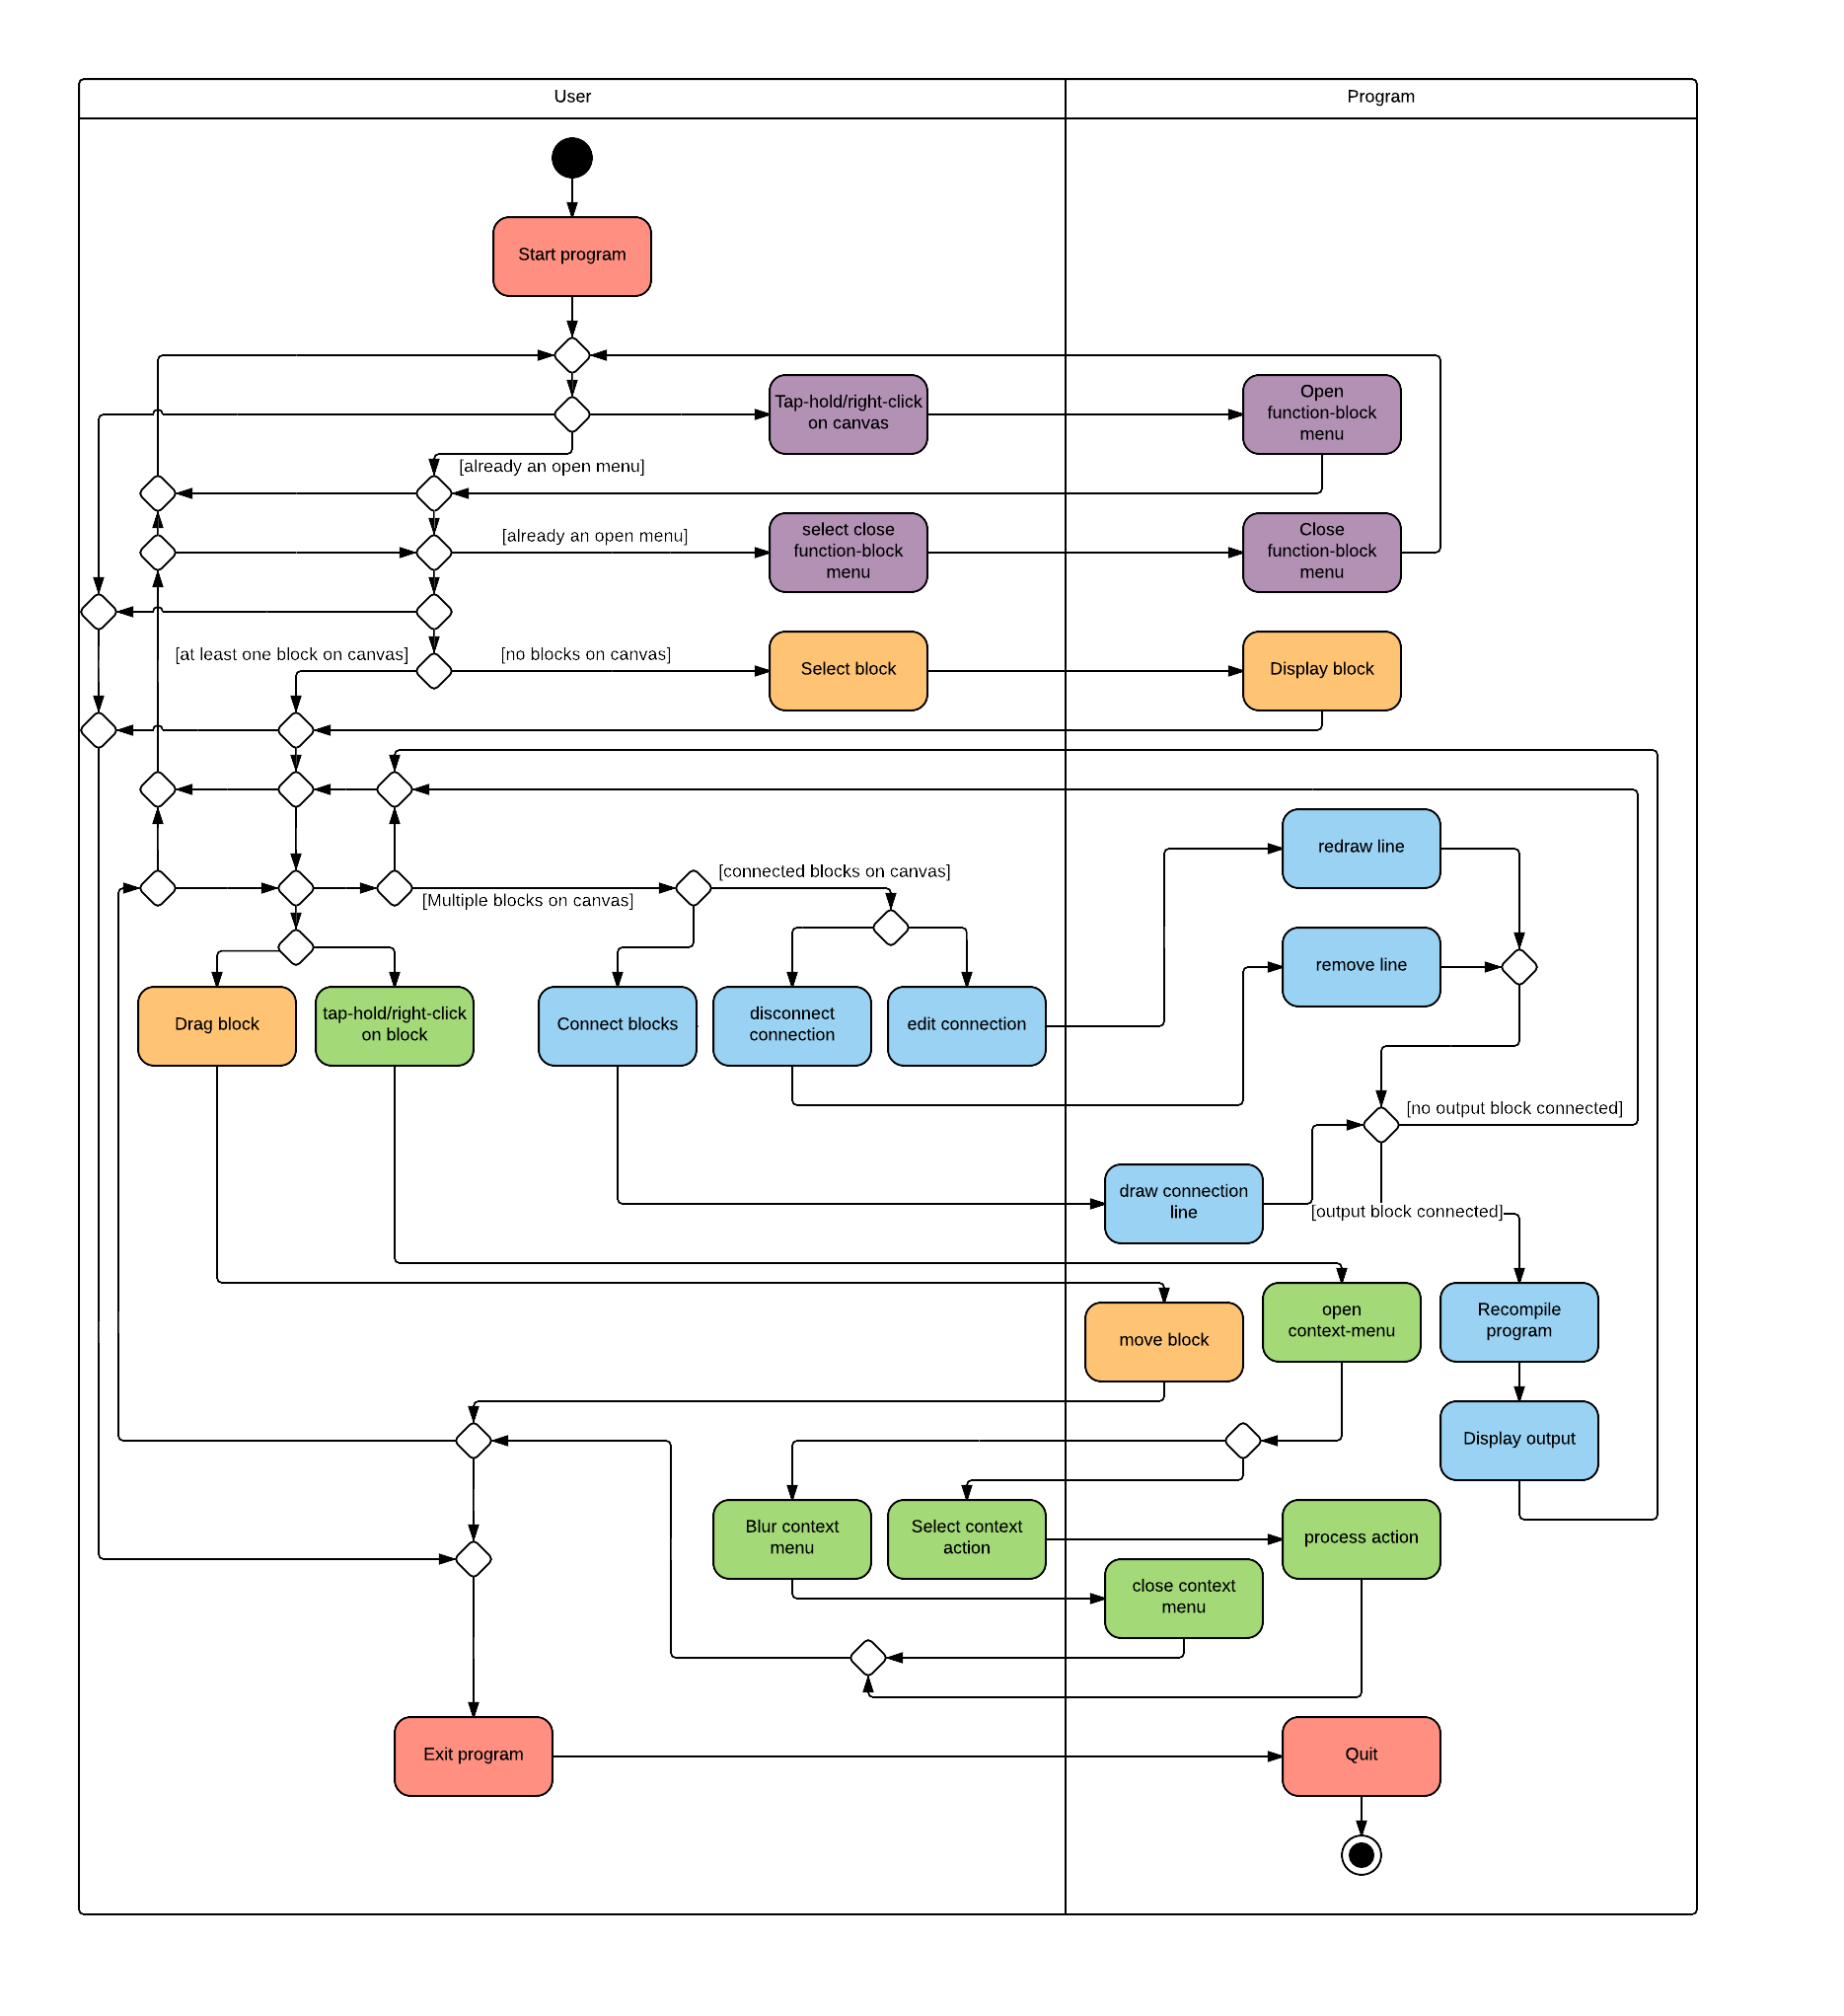
\includegraphics[width=\textwidth]{Images/activitydiagram}
	\label{fig:activitydiagram}
	\caption{Activity diagram}
\end{figure}

\section{Languages and libraries}
Viskell is written in Java 8, which comes bundled with JavaFX. \index{JavaFX}
Java 8 is chosen because it, unlike Java 7, still receives public updates at the moment of writing.
Language level 8 is chosen to make use of some of the new features in this version.
% redundant

Viskell uses TactileFX, a JavaFX touch screen library developed at the University of Twente.
The client wanted the program to use this library, which also means that Viskell had to use Java and JavaFX.

Furthermore, the following libraries have been used:

\begin{itemize}
	\item Antlr 4 (\url{http://www.antlr.org/})
	\item Guava (\url{https://github.com/google/guava})
	\item JFXtras (\url{http://jfxtras.org/})
\end{itemize}

\section{High-level architecture}
Viskell consists of two parts, a front end and a back end. \index{front end} \index{back end}
The front end is responsible for providing a user interface, handling user input, displaying error messages, and communicating with the back end.
The back end consists of a representation for Haskell code in Java, an interface to GHCi (see \ref{GHCi} on page \pageref{GHCi}) and functionality to make working with the back end easier.
This separation is made to make development and debugging for the part that generates Haskell code easier.
It also makes using the user interface for a different purpose a bit easier, although the user interface has been designed specifically for our use case.

\section{Front end architecture}
We designed Viskell with multi-touch interfaces in mind. \code{\gls{TactileAPI}}, a public library, was made available to us to assist with multi-touch interfacing. Since TactileAPI is based on javaFX, Viskell is also based on javaFX. \code{CustomUIPane}, our extension of \code{TactilePane}, has many of the same responsibilities of a main \code{Window} and stores most of the program state.
Listeners are attached to \code{CustomUIPane} to monitor \code{Mouse-} and \code{TouchEvents} that are directly responsible for the interaction with Menus.

While the general listeners are controlled from the \code{CustomUIPane}, components often have specific listeners attached to them.
This is done so that the gestures could easily change the state of the component it belonged to. Wherever possible, complex handlers were given their own class such as \code{AnchorHandler}. Since the project is aimed at providing support for multi-touch we needed additional functionality to accommodate this. A solution that is often chosen is the mapping of an input identifier to performed actions.

Placed on \code{CustomUIPane} are components, detailed further on. For all of the Components we made use of the FXML language available in javaFX.

\subsection{Components}
Basically everything visible on the \code{CustomUIPane} are components of some kind (menus fall in somewhere in-between component and non-component).
Each component is made by extending an existing javaFX \code{Node}, this is done in order to be able to directly link interactivity to the objects that are visible on the screen.
Putting each object in a separate component also added modularity and made it more easily extendible.

Most components can be categorized in 3 classes: blocks, anchors and lines.
\code{Blocks} can be further categorized into \code{FunctionBlocks}, \code{InputBlocks} and \code{OutputBlocks}.

\code{InputBlocks}, blocks that can receive input, and \code{OutputBlocks}, blocks that provide output, each have their own interface that a \code{Block} can implement. \code{DisplayBlock} is an example of such an \code{InputBlock}, \code{ValueBlock} is an example of an \code{OutputBlock}, \code{FunctionBlocks} implement both interfaces.

%TODO menus

\subsection{FXML \& CSS}
FXML is used in an attempt to separate structure from behaviour, this separation turned out to be very hard to keep. The end result is that FXML is used to construct most components were the code adds or changes the component after being loaded from FXML. We did use FXML to set most of the (often arbitrary) UI settings like height, width and other attributes.

CSS is used to separate style from structure, this separation turned out to be easier to keep. We defined the visual look (such as colours) of the entire UI in style classes in a single CSS file. Fitting style classes are applied to each component, mostly using FXML. Some style classes are updated dynamically (such as the error style class), this is done in Java.

\section{Back end architecture}

A result of our design choices is that our Java program needs to have a basic understanding of the Haskell programming
language. For this purpose we implemented two tree structures - one for expressions, one for types - supported by an
interface for GHCi, a type signature parser and a catalog.

\subsection{Communication with GHCi}
\label{GHCi}
\index{GHCi}

The base of the back-end is an interface for communication with GHCi. This interface allows us to run Haskell code
generated by the users of our application. As implementing a complete type checker for Haskell is a major challenge this
interface can also be used to check a program for faults.

\subsection{Type system and type checker}

The error messages from GHCi are hard to parse and do not always provide detailed information about where the error
occurred. Therefore we implemented our own type checker. This type checker is designed to catch most of the type errors \index{type checker}
which are in the design scope of the project and not raise false negatives. Pushing Haskell code to GHCi is still needed
to be sure that the code compiles (and will always be needed to catch runtime errors).

Internally Haskell types are represented as instances of a class. These instances can be tied together to form a
tree-like structure. This approach is chosen because it is easy to work with class instances and nested types form
a tree-like structure. \index{type tree}

An Antlr parser has been created to parse Haskell type signatures into our representation. This makes the catalog and interpreting types from GHCi easier.

The type checker is implemented using Hindley-Milner type inference. We use this algorithm to (try to) unify two
types. If the types cannot be unified, there exists a type error. The algorithm is described in detail in
\cite{borisov}. \index{Hindley-Milner} \index{type inference}

\subsection{Expressions}

Haskell expressions are represented in a tree.
By design each function can have only one argument.
Functions with more arguments are represented as a function with a single argument that produces another function with the other arguments.
Each expression holds its type including the types from the lower part of the expression tree. The root of the
expression tree therefore always knows the type of the whole tree.

Function application can be done using a special kind of expression.
This is done so function application does not directly modify other expressions in the tree.
This allows for easy changes in the front end.
Types of expressions can be updated on-the-fly taking into account the types that are applied to the arguments of functions.

Custom functions can be created using a function expression.
A function expression has an expression sub tree for the function body and a number of function arguments.
The function arguments can be used in the expression to pass the input.

The expressions that are available in the application are stored in a catalog. This catalog contains functions that are
by default available in Haskell and are known to work with the application.
